\documentclass[a4paper,11pt]{article}
\usepackage{graphicx}
\usepackage[utf8]{inputenc}
\usepackage{hyperref}

\usepackage{minted}

\begin{document}

\title{
  \textbf{Introduction Task Report.}
}
\author{Adrian Jonsson Sjödin}
\date{Fall 2022}

\maketitle

\section*{Introduction}

The purpose of this task is to determine the time efficiency of three different operations
over an array of elements, as well as familiarizing oneself with writing a report in \LaTeX.

The three operations are:
\begin{itemize}
  \item Random access: reading or writing a value at a random location in an array.
  \item Search: searching through an array looking for an item.
  \item Duplicates: finding all common values in two arrays.
\end{itemize}

\section*{Task 1}

Set up a benchmark where the access method is called on a larger and larger array of size
\textit{n} and present your conclusions and observations on how much time is needed for a reading
of a value at a random location in the array.

\section*{Method}

To be able to measure the time it takes for one random access of an array of size
\textit{n}, I used the provided code from the task with some modifications. Mainly I adjusted
it so that the number of times we searched for an element in the array is not the same as
the size of the array. Instead we input the size of the array (\textit{n}) and the nr of
searches into the method call:

\begin{minted}{java}
  private static double access(int arraySize, int nrOfSearches) {
    int k = 1_000_000;
    int l = nrOfSearches;
   /* code here*/
  }
\end{minted}

This method will then return a time in nano seconds for the average time of one random array
access.

\section*{Result}

\begin{table}[h]
  \begin{center}
    \begin{tabular}{|c|c|c|}
      \hline
      \textbf{Array size} & \textbf{Nr. of searches} & \textbf{Time in ns} \\
      \hline
      10                  & 10 000                   & 0.86                \\
      100                 & 10 000                   & 0.26                \\
      1000                & 10 000                   & 0.26                \\
      10 000              & 10 000                   & 0.31                \\
      50 000              & 50 000                   & 0.50                \\
      100 000             & 10 000                   & 0.72                \\
      \hline
    \end{tabular}
    \caption{Output from the program being run once}
    \label{tab:task1}
  \end{center}
\end{table}


\section*{Discussion}

It seems like the time to access a random element in an array of
size \textit{n} increases with the size of the array, which I think is expected.
The time increase does not seem to be linear but rather a slower time increase than
that, which if true is good. However the trustworthiness of this result is
questionable since every time I ran the program it gave me quite different results,
where sometimes the time being lower and lower for larger \textit{n}, and other times
having one of the times in the middle being drastically larger than the rest.

I don't know if the reason behind this fluctuation of the time results are buggy code, or
if it is something that Java does behind the scenes that could somehow change the results.
It makes more sense that the reason lies in the code since one would think that whatever
Java might do behind the scenes should be consistent and thus not influence the results.
But even then I can't find where the problem would lie in the code which leads me to believe
that the reasons has to be connected to the randomness of the accessing somehow.

\section*{Task 2}

Search through an array for an element and benchmark how the time to find said element changes for bigger and bigger arrays. 

\section*{Method}

I used the code provided by the teacher and made sure to pick $m > n$ as instructed in the task. I settled for $m = 100 000$ and $k = 1000$.
 Filling in the code in the section left blank with what seemed appropriate I arrived to the result seen in the section bellow. 

\section*{Result}

\begin{figure}[h]
  \begin{center}
    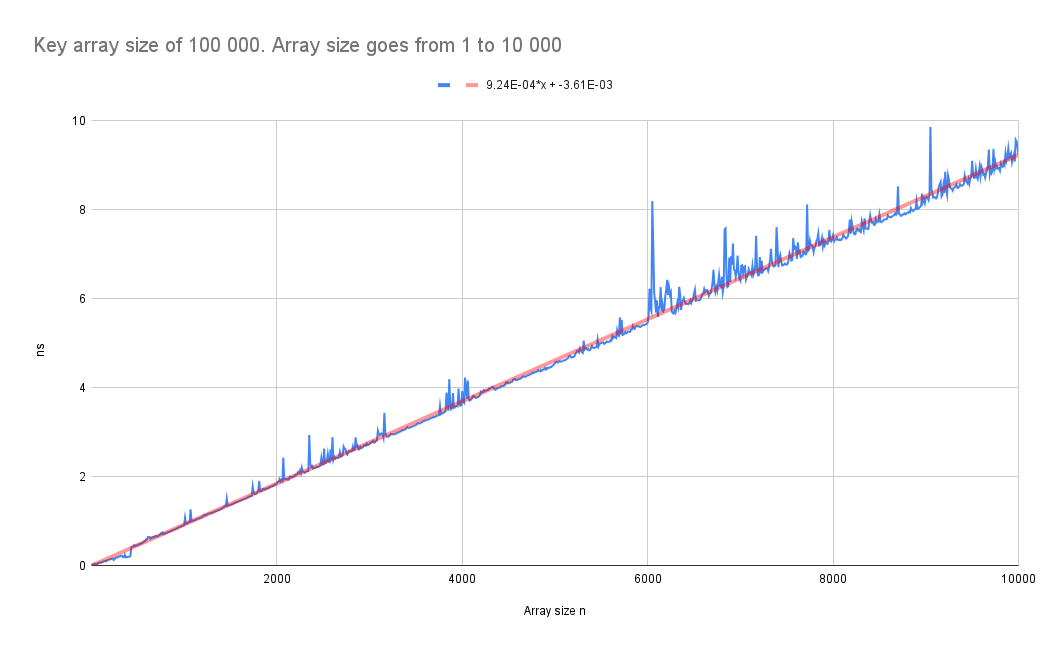
\includegraphics[width=\textwidth]{task2dataPlot.png}
    \caption{Time taken per element search when array size $n \to 10,000$}
    \label{fig:task2}
  \end{center}
\end{figure}

\section*{Discussion}

It seems like the time taken to search for en element within an array increases linearly with the size of the array. However after we passes around $n=6,000$ 
the results starts behaving quite weird fluctuating more with multiple peaks. To be completely honest I have no ide why this is. I think it could perhaps be Java's 
\textit{Just-In-Time} compiler thing that was mentioned in the task. But since I don't know how that thing works I can't say for certain that that's the problem.

Furthermore I also don't quite understand the connection between \textit{k}, \textit{m} and \textit{n} in the provided code. Changing this values affected the time
reported by the program, but not the overall linearity of it. 

\section*{Task 3}

Find duplicates in two arrays of length \textit{n}. Estimate how n you would be able to handle if you had an hour of computation time.

\section*{Method}
For this task there was no code provided by the teacher, but since the task is basically the same as in task 2, the solution only required a small modification to 
the code from task 2, mainly making sure the arrays had the same size.

\section*{Result}

\begin{figure}[h!]
  \begin{center}
    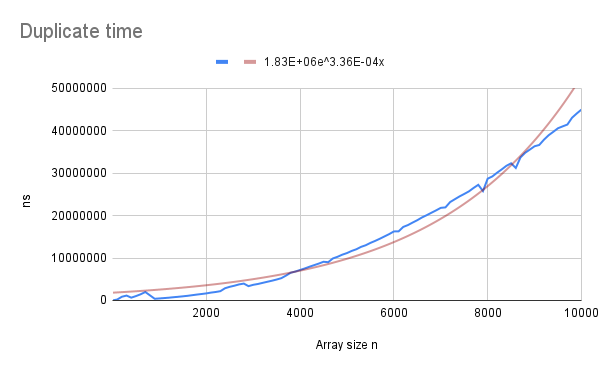
\includegraphics[width=\textwidth]{task3plot.png}
    \caption{Time taken to find all duplicates when $n\to 10,000$}
  \end{center}
\end{figure}

\section*{Discussion}
To be completely honest I didn't understand exactly what the difference was between this task and task 2 since it seemed like you asked us to check the same thing.
In task 2. You ask us to search for a an element in an array by using a key array that contains random elements. In task 3 you ask us to search for elements that 
are in both arrays. The only difference seemed to be the array size. I'm assuming I missed something when doing this task but I've asked a lot of other people taking
the course and they seemed as lost as me when it came to these tasks. My conclusion on task 3 is thus that I can't reach any conclusions since I don't really 
understand what you're asking for and I'm pretty sure that the result seen in figure 2 is misleading. 

Reflecting back on these task there aren't really anything I could have done differently. I've spent probably around 18 hours on this assignment and I feel that even 
if I had double that time left I would still be stuck. The problem is simply that I, and everyone else I've asked (10+ people) simply don't understand your instruction, 
what are feasible results and the theory behind it.\\

Link to code \hyperlink{https://github.com/adrian-jonsson-sjoedin/ID1021-AlgoData/blob/main/ArrayTimes/src/Main.java}{GitHub}


\end{document}
